\section{Automatic Image Processing}

In this section we provide detailed hands-on instruction on automatic image processing within 2dx \cite{scherer20142dx_automator}, including on-the-fly image drift-correction. The here described pipeline is optimised for data recorded on a direct electron detector, such as the Gatan K2 summit. 

\subsection{Real-time motion-correction}

In case you record dose fractioned movies we propose the drift-correct them on-the-fly as described in:

\textit{https://github.com/C-CINA/2dx/wiki/Automatic-Drift-Correction-C-CINA-setup}

Additionally instruction about setting up our automatic drift-correction pipeline is available under:

\textit{https://github.com/C-CINA/2dx/wiki/Automated-Drift-Correction-GUI}

2dx\_automator will later be used to automatically process the drift-corrected average of all frames.

\subsection{Required software}

2dx\_automator is only supported under Linux right now.
Please make sure that the list of dependencies is installed on the used system.

\begin{itemize}
	\item \texttt{TkInter} a python GUI package
	\item \texttt{py-thread} to be able to dispatch processing into different tasks
	\item \texttt{py-imaging (aka PIL)} the python image processing libraries
	\item \texttt{eman2/sparx} has to be installed and sourced on the system
	\item \texttt{py-matplotlib} to generate plots
	\item \texttt{py-shutil} for low-level operating system interaction
	\item \texttt{ImageMagic} especially the command-line tool \texttt{convert} has to be available
\end{itemize}

Additionally 2dx\_automator requires that \texttt{2dx\_image, 2dx\_merge} are available in the command line. If you installed a pre-compiled package please add 2dx's binary directory to your path:

\texttt{export PATH = /opt/2dx/bin:\$PATH}

If you compiled the software from source directly on your computer you should source the installation-binary folder as well:

\texttt{export PATH = <your\_install\_dir>/bin:\$PATH}

where \texttt{<your\_install\_dir>} equals the second argument passed to the \texttt{build\_all}-script. If you did not pass any argument to the build-script then \texttt{<your\_install\_dir>} equals \texttt{\textasciitilde{}/2dx/}.

\subsection{Automation setup}

\subsection{2dx\_automator}

asdf  \autoref{fig:auto} adf.

\begin{figure}
	\centering
	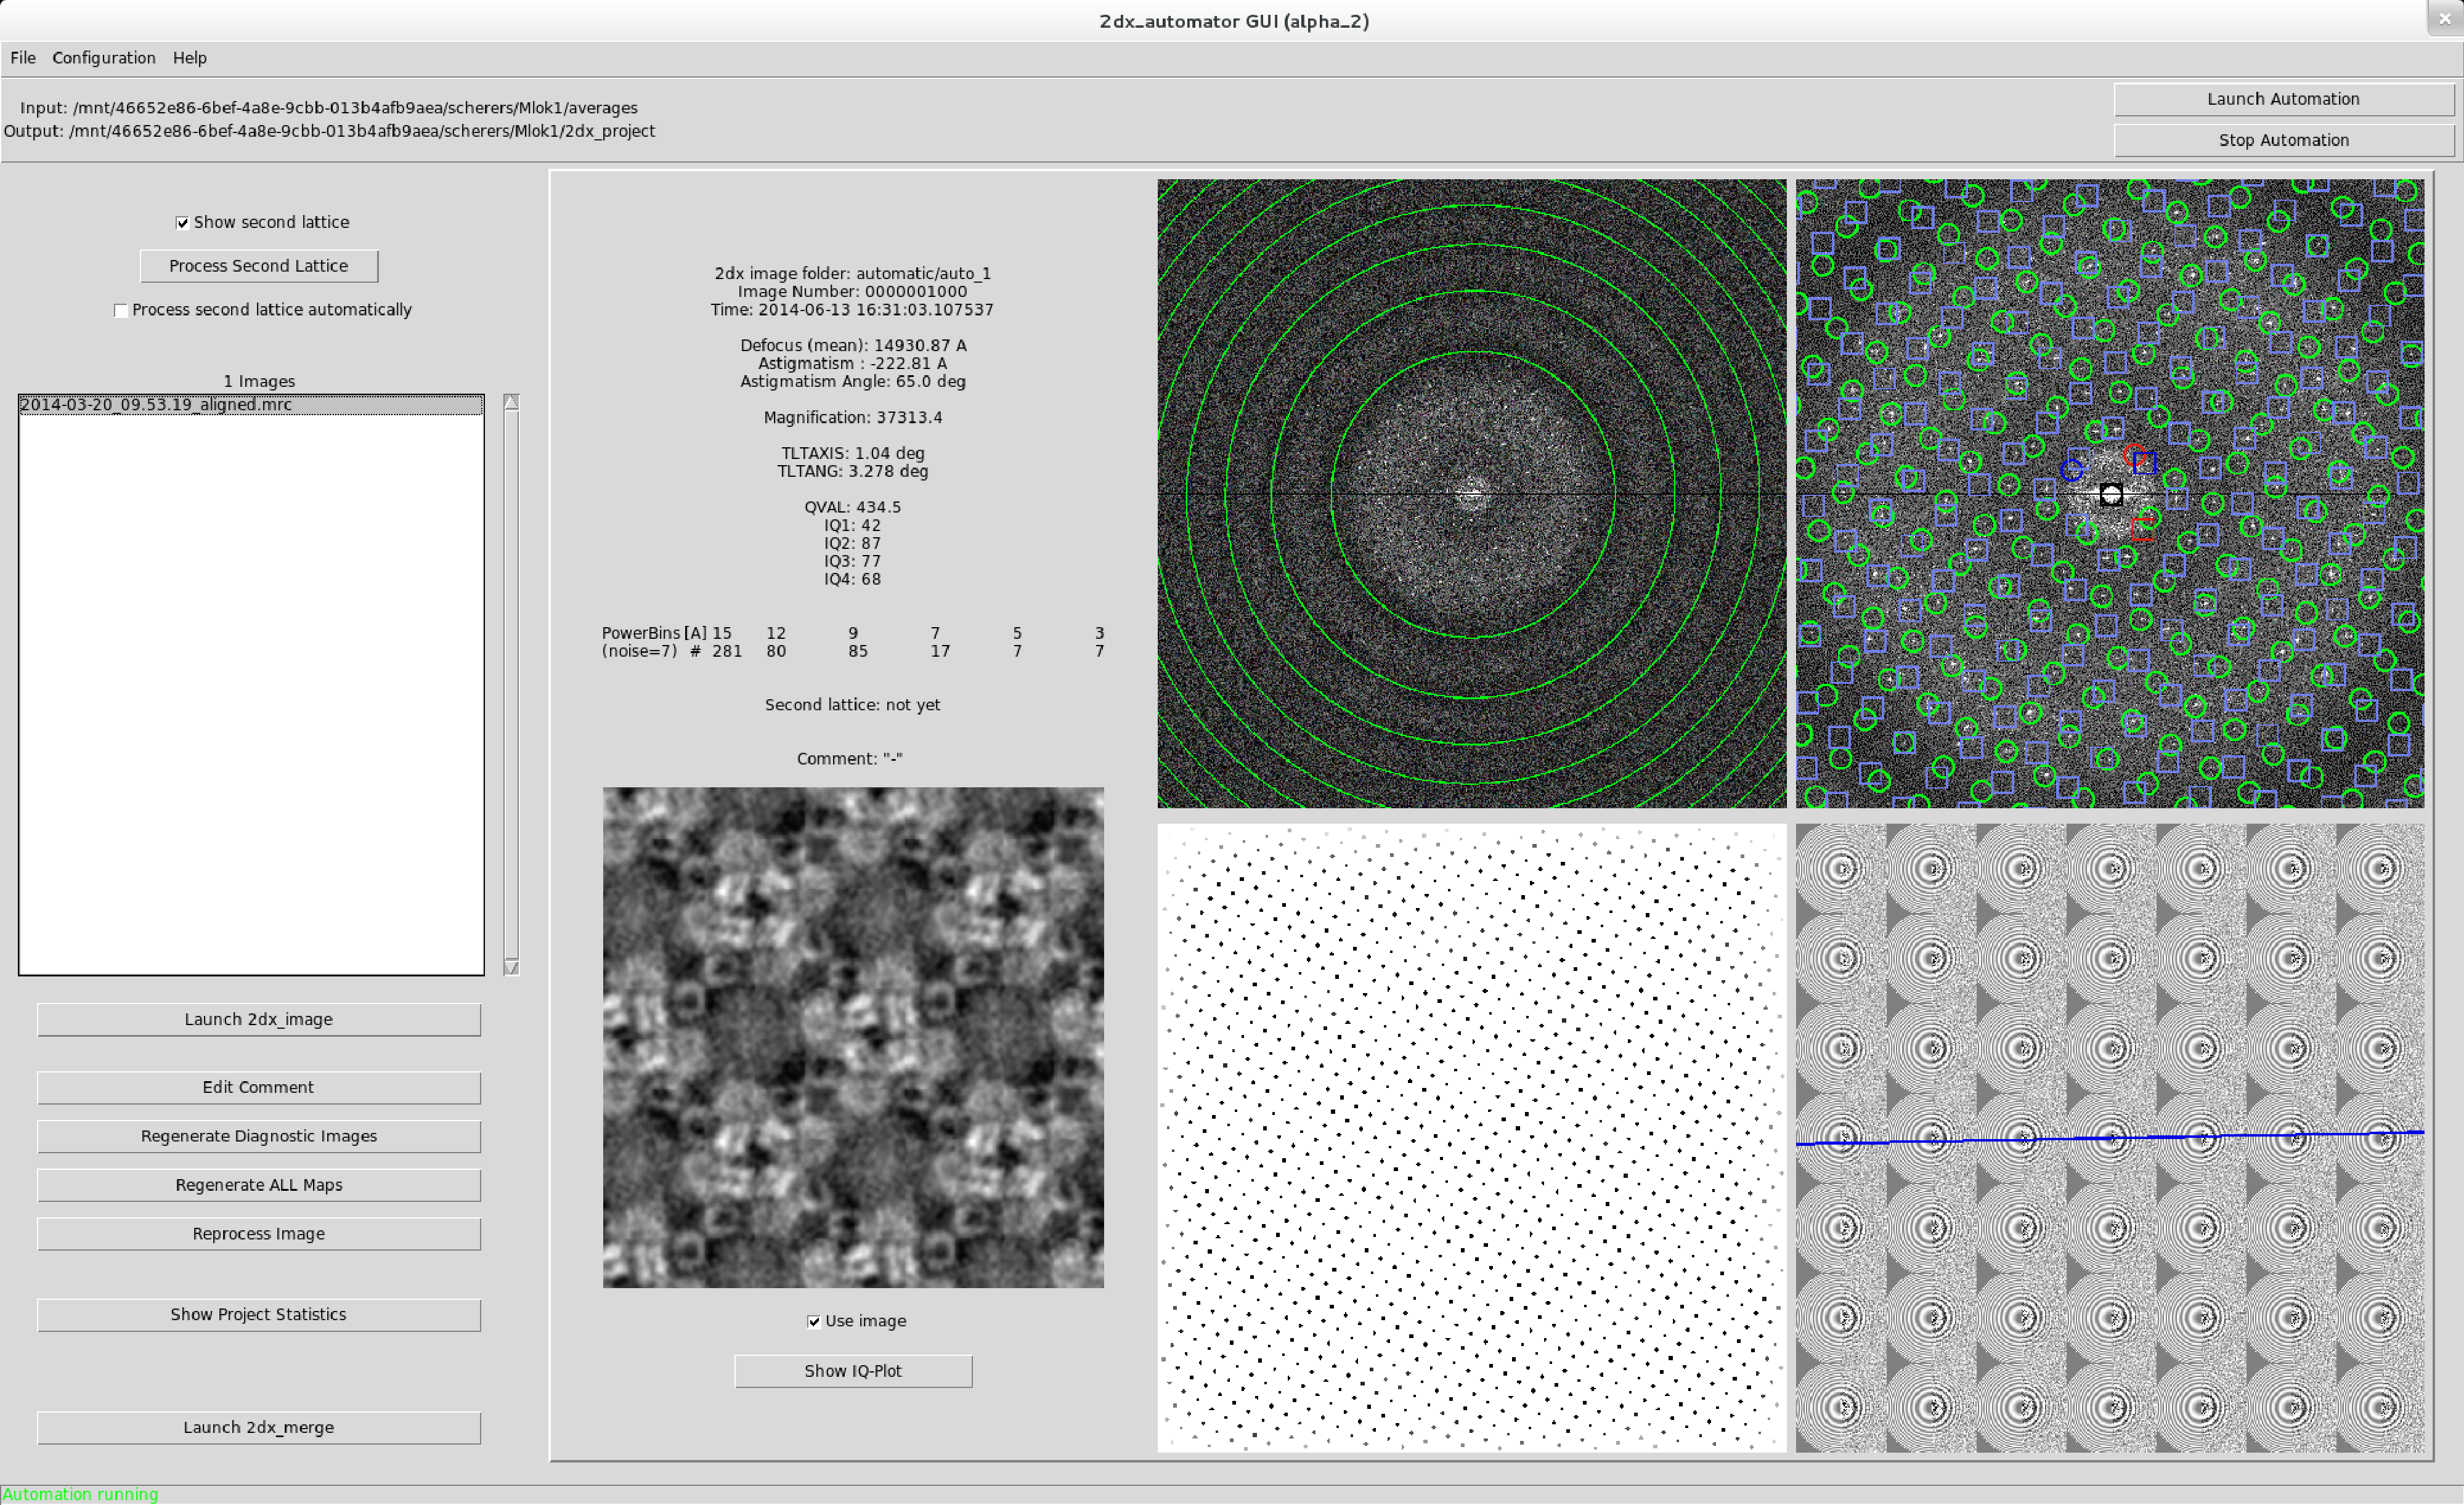
\includegraphics[width=1.0\textwidth]{auto.pdf}
	\caption{2dx\_automator}
	\label{fig:auto}
\end{figure}

\begin{figure}
	\centering
	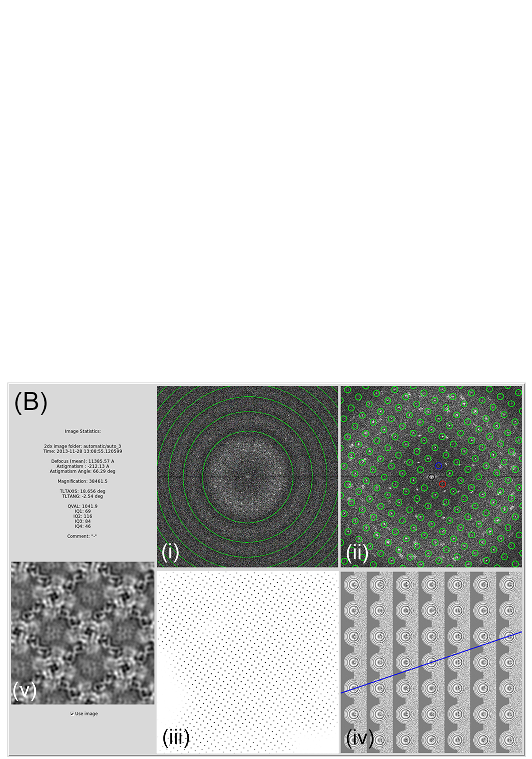
\includegraphics[width=1.0\textwidth]{auto2.pdf}
	\caption{Diagnostic view of the 2dx\_automator GUI. (i) Fourier transform with Thon rings and (ii) fitted lattice, (iii) peak profile from the unbending step used to mask the image, (iv) locally estimated defocus values, (v) final 2D projection map.}
	\label{fig:auto2}
\end{figure}


\subsection{Advanced tricks}

\begin{description}
	\item [Second lattice processing]
	\item [Manual processing intervention] 
	\item [Comment editing]
	\item [Updating image maps]
	\item [Reprocess an image]
	\item [Project statistics]
	\item [IQ-Stat analysis]
	\item [Configuration file handling] 
\end{description}



\begin{figure}
	\centering
	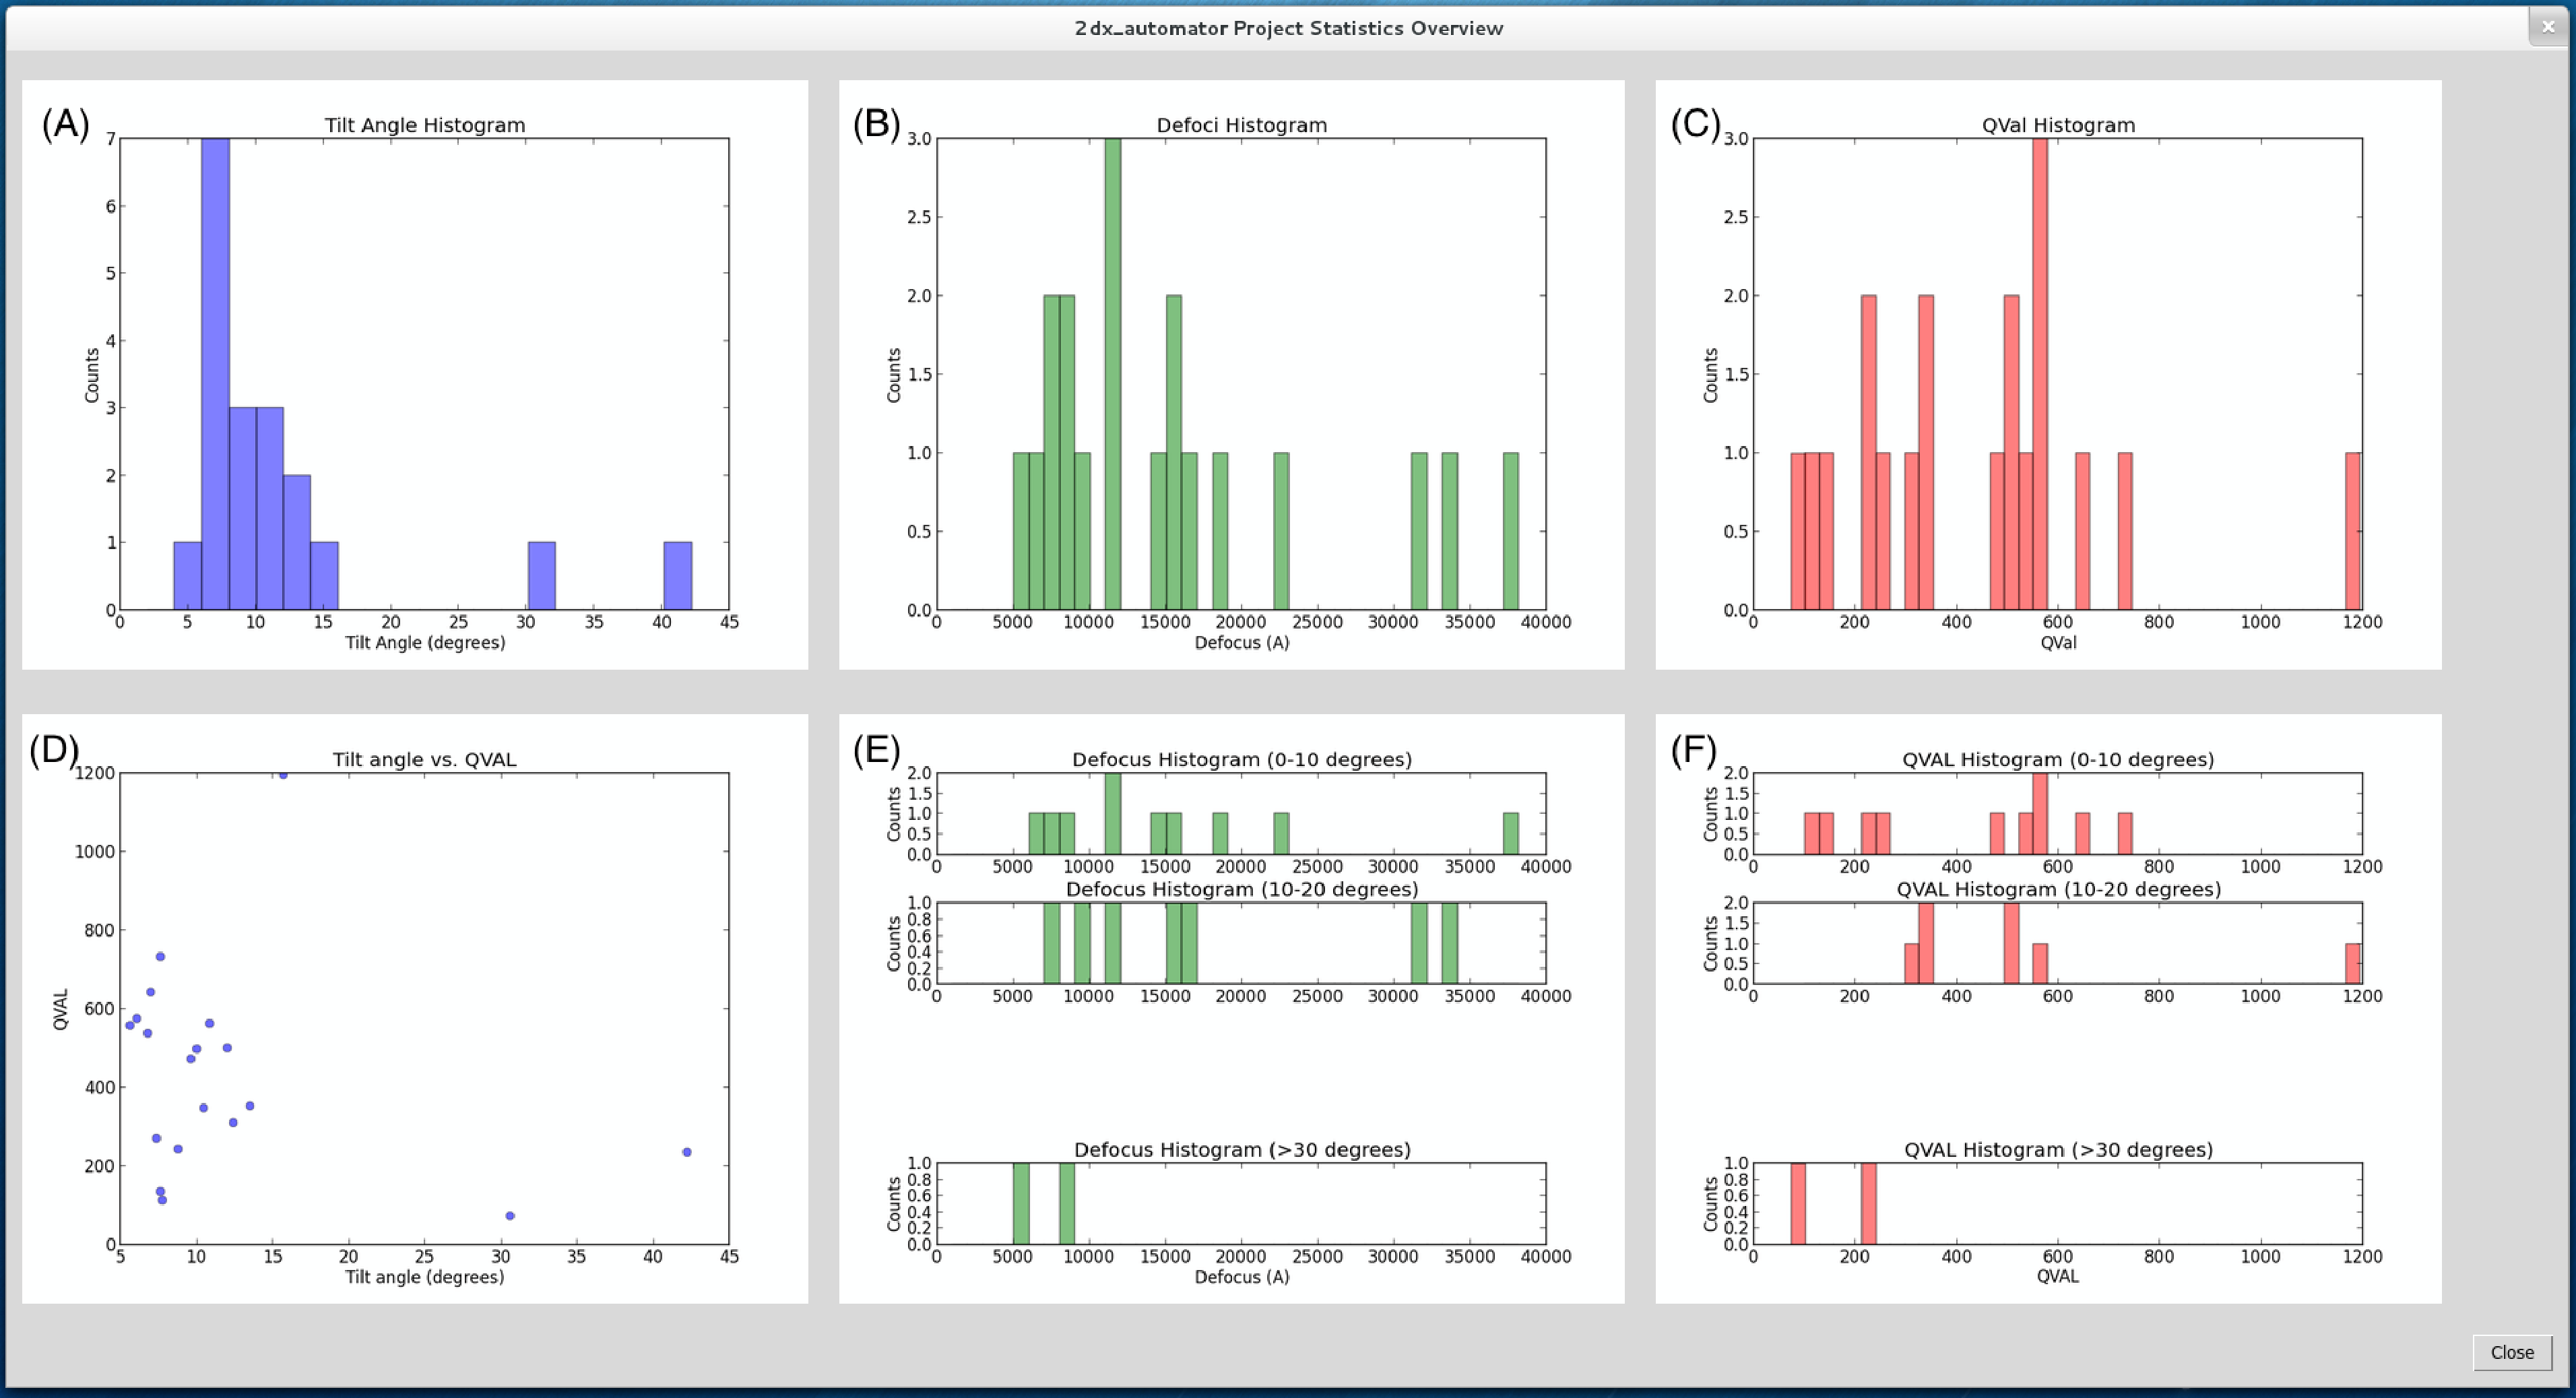
\includegraphics[width=1.0\textwidth]{auto_overview.pdf}
	\caption{Project stat}
	\label{fig:auto_stat}
\end{figure}